\documentclass[11pt,a4paper,oneside]{book}
\usepackage[T1]{fontenc}
\usepackage[utf8]{inputenc}
\usepackage{lmodern}
\usepackage[a4paper,margin=24mm,headheight=15pt]{geometry}
\usepackage{microtype}
\usepackage{amsmath,amssymb,mathtools}
\usepackage{booktabs,longtable,tabularx,array,multirow}
\usepackage{graphicx}
\usepackage{xcolor}
\usepackage{hyperref}
\usepackage{bookmark}
\usepackage{fancyhdr}
\usepackage{enumitem}
\usepackage{listings}
\usepackage{caption}
\usepackage{float}
\usepackage{pdflscape}
\usepackage{tikz}
\usetikzlibrary{positioning}
\usepackage{url}
\usepackage{titlesec}
\usepackage{etoolbox}
\usepackage{lastpage}

\definecolor{navy}{HTML}{12304A}
\definecolor{teal}{HTML}{157A78}
\definecolor{amber}{HTML}{B36A00}
\definecolor{softgray}{HTML}{F1F4F6}
\definecolor{darkgray}{HTML}{40464D}
\definecolor{riskred}{HTML}{8C2F39}

\hypersetup{
  colorlinks=true,
  linkcolor=navy,
  citecolor=teal,
  urlcolor=teal,
  pdftitle={NHDF-CCD Cradle-to-Grave v0.5},
  pdfauthor={Tom Klootwijk, attribution as supplied; engineering continuation prepared 2026-09-01},
  pdfsubject={Continuous collision detection formalization, implementation, validation, and lifecycle dossier},
  pdfkeywords={CCD, continuous collision detection, vertex-face, edge-edge, collision certificates, NHDF}
}

\pagestyle{fancy}
\fancyhf{}
\fancyhead[L]{\small NHDF--CCD v0.5}
\fancyhead[R]{\small Cradle-to-Grave Dossier}
\fancyfoot[L]{\small Research reference --- not production safety certification}
\fancyfoot[R]{\small \thepage\ / \pageref{LastPage}}
\renewcommand{\headrulewidth}{0.3pt}
\renewcommand{\footrulewidth}{0.3pt}

\titleformat{\chapter}[display]
  {\normalfont\bfseries\color{navy}}
  {\filleft\Large\chaptertitlename\ \thechapter}
  {1ex}
  {\titlerule\vspace{1ex}\Huge}
\titleformat{\section}{\Large\bfseries\color{navy}}{\thesection}{0.7em}{}
\titleformat{\subsection}{\large\bfseries\color{teal}}{\thesubsection}{0.7em}{}

\setlist{nosep,leftmargin=1.6em}
\setlength{\parindent}{0pt}
\setlength{\parskip}{0.55em}
\setcounter{tocdepth}{2}
\setcounter{secnumdepth}{3}

\lstdefinestyle{code}{
  basicstyle=\ttfamily\footnotesize,
  breaklines=true,
  frame=single,
  backgroundcolor=\color{softgray},
  rulecolor=\color{darkgray},
  numbers=left,
  numberstyle=\tiny\color{darkgray},
  xleftmargin=1.5em,
  framexleftmargin=1.2em,
  showstringspaces=false,
  columns=fullflexible,
  keepspaces=true
}
\lstset{style=code}

\newcommand{\status}[1]{\texttt{#1}}
\newcommand{\claim}[1]{\textbf{Claim:} #1}
\newcommand{\evidence}[1]{\textbf{Evidence:} #1}
\newcommand{\boundary}[1]{\textbf{Boundary:} #1}
\newcommand{\risk}[1]{\textcolor{riskred}{\textbf{#1}}}
\newcommand{\release}{NHDF--CCD v0.5}
\input{generated_values.tex}

\begin{document}

\begin{titlepage}
\pagecolor{navy}\color{white}
\centering
\vspace*{22mm}
{\Huge\bfseries NHDF--CCD\\[4mm] Cradle-to-Grave v0.5\par}
\vspace{8mm}
{\Large Feature Contact, Rigid-Motion Bounds, Event Grouping, Response Boundary, and Public-Corpus Validation\par}
\vspace{18mm}
\begin{tikzpicture}[scale=1.0]
  \draw[white,very thick] (0,0) -- (12,0);
  \foreach \x/\lab in {0/State,2/Bounds,4/Candidates,6/Roots,8/Certificate,10/Event,12/Policy}{
    \fill[white] (\x,0) circle (0.11);
    \node[white,align=center,font=\small] at (\x,-0.55) {\lab};
  }
  \draw[white,thick,->] (2.2,1.0) arc[start angle=165,end angle=15,x radius=3.8,y radius=0.9];
  \node[white,font=\small] at (6,2.0) {deterministic feedback and replay};
\end{tikzpicture}
\vfill
\begin{tabular}{rl}
Primary attribution: & Tom Klootwijk (as supplied in source materials)\\
Release date: & \ReleaseDate\\
Specification state: & research reference / validation gate C1+\\
Scope: & literal computer-graphics and physics-engine CCD\\
Privacy note: & new release metadata omits supplied civil identifiers\\
\end{tabular}
\vspace{16mm}

{\small This dossier is cumulative. Part I documents the v0.5 continuation; the preserved v0.4 baseline follows as Part II in the delivered PDF. No medical, quantum, optical, chemical, biological, or cosmological claim is promoted by the CCD results.}
\end{titlepage}
\nopagecolor\color{black}

\frontmatter
\chapter*{Release statement}
\addcontentsline{toc}{chapter}{Release statement}

This release continues the earlier roadmap by turning from a primitive-only CCD nucleus toward the feature queries required by triangle-based graphics engines. It adds linearly moving vertex--face and edge--edge queries, conservative handling of persistent coplanarity, rigid-motion speed envelopes, deterministic grouping of overlapping time-of-impact intervals, a restricted response example, and a locally vendored public-corpus harness.

The work is deliberately narrower than an ``entire substrate'' claim. The non-CCD materials are retained as separately testable adapters; they do not inherit validity from collision tests. The central scientific discipline is unchanged: a result that cannot be certified within the stated model and resource budget remains \status{INCONCLUSIVE}, \status{RESOURCE\_EXHAUSTED}, \status{UNSUPPORTED}, or a numerical failure. It is never silently rewritten as \status{MISS}.

\begin{center}
\begin{tabularx}{0.94\textwidth}{>{\bfseries}p{0.22\textwidth}X}
\toprule
Release axis & v0.5 position\\
\midrule
Geometry & affine vertex--face and edge--edge; primitive v0.4 baseline preserved\\
Correctness device & cubic candidate equation plus closed-feature witness; conservative distance fallback\\
Time semantics & normalized interval $t\in[0,1]$ with lower and upper TOI bounds\\
Failure semantics & explicit, typed, capacity-aware, replayable\\
External evidence & two vendored adversarial Sample-Queries files with original README and MIT license\\
Response & frictionless translational impulse example only; not a production manifold solver\\
Acceleration & CUDA coefficient-stage skeleton only; no GPU conformance claim\\
Lifecycle & provenance through retirement, with manifests and release validation log\\
\bottomrule
\end{tabularx}
\end{center}

\chapter*{Executive findings}
\addcontentsline{toc}{chapter}{Executive findings}

\claim{The v0.5 implementation materially advances the CCD center of gravity.} It handles the two canonical linear mesh feature pairs, returns geometric witnesses, groups time intervals into deterministic events, and provides public-corpus ingestion rather than relying only on bespoke examples.

\evidence{The release executed \PythonTests\ Python tests, one compiled C++17 smoke test, \SyntheticTotalQueries\ seeded synthetic feature queries, \RigidSamples\ rigid-bound inequality samples, \ResponseSamples\ response audits, and two complete vendored CSV files.} The raw records, environment, source, figures, and scripts are included in the ZIP.

\claim{Endpoint sampling remains demonstrably insufficient.} In the constructed tunnelling corpus it missed \SyntheticVFEndpointMisses\ vertex--face contacts and \SyntheticEEEndpointMisses\ edge--edge contacts that occurred between the endpoints of the step.

\boundary{The feature solver is not yet exact arithmetic.} It uses double-precision cubic root finding, tolerance-based root acceptance, and a bounded fallback for persistent or ill-conditioned coplanarity. Public-corpus mismatches and inconclusive results are retained in the evidence tables and CSV files. They are defects or open cases to be addressed, not values to hide.

\claim{The response layer is intentionally subordinate to detection.} Momentum and non-energy-gain audits exercise a simple frictionless translational impulse, but angular impulses, friction, stacking, stabilization, manifold solve, and long-horizon dynamics remain outside the validated scope.

\chapter*{How to read this dossier}
\addcontentsline{toc}{chapter}{How to read this dossier}

Chapters~1--4 define the claim, model, and proof obligations. Chapters~5--9 document feature algorithms, bounds, events, and response. Chapters~10--13 describe the external corpus, validation results, software implementation, and engine integration. Chapters~14--18 complete the lifecycle, adapter separation, risk case, roadmap, and retirement policy. Appendices preserve schemas, logs, selected source listings, and a package inventory. Part II is the unmodified v0.4 PDF baseline.

A value in a result table is generated from \path{validation/validation_summary.json} unless stated otherwise. Throughput is a build-host observation and not a portable promise.

\tableofcontents
\listoffigures
\listoftables

\mainmatter

\chapter{Problem and claim boundary}
\section{Literal CCD problem}

For two time-dependent closed sets $A(t)$ and $B(t)$ over a simulation step, continuous collision detection asks whether
\[
  \exists t\in[0,1] : A(t)\cap B(t)\neq\varnothing,
\]
and, when possible, asks for the earliest contact time or a conservative interval containing it. A production engine additionally needs feature identity, witness geometry, simultaneous-event policy, bounded execution, and a rule for uncertainty.

The v0.5 feature profile restricts every supplied endpoint to affine motion,
\[
  x(t)=x_0+t(x_1-x_0).
\]
This is the common linearized per-step model used by mesh CCD pipelines. It is not an assertion that the physical world is globally affine; it is a declared numerical profile.

\section{What is claimed}

Within the declared profile, the reference implementation can:
\begin{itemize}
  \item generate cubic coplanarity candidates for vertex--face and edge--edge queries;
  \item reject candidates that fail closed-feature containment or distance checks;
  \item fall back to a distance-rate-bounded interval search when coplanarity is persistent or ill-conditioned;
  \item report typed certificates and deterministic event groups;
  \item parse exact-rational public query files without discarding their labels.
\end{itemize}

\section{What is not claimed}

The release does not establish an exact-predicate solver, a complete rotating or deformable mesh pipeline, global physical stability, GPU equivalence, a production contact response, or a universal physical substrate. The same notation may be used by future adapters, but notation is not constitutive physics.

\section{Conformance position}

The original ladder separated symbolic specification, deterministic CPU reference, verified GPU runtime, application advantage, and physical substrate. v0.5 advances the deterministic CPU reference for feature CCD and its evidence harness. It does not cross the verified-GPU gate.

\chapter{Typed state and result semantics}
\section{State threading}

The operator chain is treated as a transformation of an enriched state rather than as a composition of incompatible scalar objects. For CCD, a compact state is
\[
\Sigma_n=(S_n,L_n,C_n,Q_n,R_n,E_n,T_n),
\]
where $S_n$ is the immutable scene snapshot, $L_n$ the logical time identity, $C_n$ broad-phase candidates, $Q_n$ typed feature queries, $R_n$ result certificates, $E_n$ grouped events, and $T_n$ telemetry. Each stage has signature $O_j:\Sigma\rightarrow\Sigma$.

\section{Status algebra}

\begin{table}[H]
\centering
\caption{Result statuses and mandatory host interpretation}
\begin{tabularx}{\textwidth}{>{\ttfamily}p{0.24\textwidth}X}
\toprule
HIT & A contact was found and an upper TOI bound plus witness is supplied.\\
INITIAL\_OVERLAP & The features are already within tolerance at $t=0$.\\
MISS & The declared method certified no contact in the normalized step.\\
INCONCLUSIVE & The current method/budget could not establish hit or miss.\\
RESOURCE\_EXHAUSTED & A finite queue, interval, or iteration budget ended first.\\
UNSUPPORTED & The query lies outside the declared geometry/motion profile.\\
NUMERICAL\_FAILURE & Non-finite input or arithmetic invalidated the result.\\
\bottomrule
\end{tabularx}
\end{table}

Only \status{MISS} authorizes free motion under the solver contract. A host may choose a conservative degraded policy for other non-contact statuses, but it may not relabel them without recording that policy.

\section{Certificate integrity}

Every certificate can be serialized canonically and hashed. The digest is a replay locator, not a cryptographic statement about authorship. The certificate records method, termination reason, tolerance, candidate count, root condition indicator, witness data, and optional bounded trace.

\chapter{Feature geometry}
\section{Vertex--face contact}

Let $p(t)$ be a vertex and $a(t),b(t),c(t)$ the triangle vertices. Coplanarity requires
\begin{equation}
 f_{VF}(t)=\big(p(t)-a(t)\big)\cdot\Big(\big(b(t)-a(t)\big)\times\big(c(t)-a(t)\big)\Big)=0.
 \label{eq:vf}
\end{equation}
Each vector is affine, so $f_{VF}$ is at most cubic. A real root in $[0,1]$ is only a candidate. The point must also lie in the closed triangle, checked through the closest-point witness and barycentric coordinates
\[
  p^*=u a+v b+w c,\qquad u+v+w=1,\qquad u,v,w\geq0.
\]

\section{Edge--edge contact}

For edge endpoints $a_0,a_1,b_0,b_1$, the coplanarity polynomial is
\begin{equation}
 f_{EE}(t)=\big(b_0(t)-a_0(t)\big)\cdot\Big(\big(a_1(t)-a_0(t)\big)\times\big(b_1(t)-b_0(t)\big)\Big).
 \label{eq:ee}
\end{equation}
At a candidate root, closed-segment closest parameters $s,u\in[0,1]$ and the witness distance decide admissibility.

\section{Degenerate features}

Zero-area triangles, zero-length edges, parallel segments, collinearity, and persistent coplanarity are not exceptional in real meshes. Static distance routines reduce degenerate triangles to their edges and segments to points where necessary. Persistent dynamic degeneracy is routed to the interval fallback. The present fallback is conservative but may end inconclusively; exact classification remains a v0.6 objective.

\chapter{Cubic candidates and numerical conditioning}
\section{Coefficient construction}

Writing three affine vectors as $r(t)=r_0+r_1t$, $u(t)=u_0+u_1t$, and $v(t)=v_0+v_1t$, define
\[
\begin{aligned}
 c_0&=u_0\times v_0,\\
 c_1&=u_1\times v_0+u_0\times v_1,\\
 c_2&=u_1\times v_1.
\end{aligned}
\]
Then $r(t)\cdot(u(t)\times v(t))=a_0+a_1t+a_2t^2+a_3t^3$, with
\[
\begin{aligned}
 a_0&=r_0\cdot c_0,\\
 a_1&=r_1\cdot c_0+r_0\cdot c_1,\\
 a_2&=r_1\cdot c_1+r_0\cdot c_2,\\
 a_3&=r_1\cdot c_2.
\end{aligned}
\]
The same coefficient kernel serves both feature types after choosing the correct vectors.

\section{Root acceptance}

The CPU reference uses double-precision polynomial roots, retains roots whose imaginary component is below a scale-aware tolerance, clips roots slightly outside $[0,1]$, clusters near duplicates, and validates geometry at every retained root. A coefficient-ratio indicator is recorded for audit. This is useful engineering evidence but not a proof of exact root isolation.

\section{Why the geometric witness is indispensable}

Coplanarity alone has many false candidates: the point may lie outside the triangle, or the two infinite lines may intersect outside their finite segments. The witness test enforces the actual closed-feature problem. Conversely, a tolerance can merge near-contact with exact contact; therefore every release and engine integration must state its geometric scale and contact thickness.

\chapter{Persistent coplanarity and the conservative fallback}
\section{Distance-rate bound}

For moving closed sets, distance is Lipschitz with respect to their Hausdorff motion. If set $A$ has point-speed bound $V_A$ and set $B$ has bound $V_B$, then
\begin{equation}
  |d(A(t_1),B(t_1))-d(A(t_0),B(t_0))|\leq(V_A+V_B)|t_1-t_0|.
  \label{eq:lipschitz}
\end{equation}
For an affine segment or triangle, interior-point velocity is a convex combination of endpoint or vertex velocities, so the maximum endpoint/vertex speed is valid.

For an interval $I=[\ell,h]$ and a sample at $s\in I$, a lower bound is
\[
  d_I^{\min}\geq d(s)-L\max(|s-\ell|,|h-s|),\qquad L=V_A+V_B.
\]
The implementation combines endpoint and midpoint samples. An interval is discarded only when this lower bound exceeds contact thickness plus tolerance.

\section{Termination semantics}

If a sampled contact is found and every earlier interval is certified separated, the fallback returns a contact interval. If a potentially contacting interval reaches the time tolerance without a contact sample, it remains inconclusive. If the interval budget ends, the status is resource exhaustion. This design favors visible uncertainty over a false negative.

\section{Golden-ratio splitting}

Earlier NHDF materials explored golden-ratio schedules. v0.5 keeps interval policy conceptually replaceable, but the reference fallback uses deterministic midpoint subdivision. A splitting ratio has no correctness privilege; it must be compared empirically under identical proof bounds and budgets.

\chapter{Rigid-motion envelopes}
\section{Relative speed bound}

For a rigid body with center velocity $v$, angular-speed magnitude $|\omega|$, and support radius $r$, any attached point has speed bounded by
\[
  V\leq\|v\|+|\omega|r.
\]
For two bodies,
\begin{equation}
 V_{rel}\leq\|v_A-v_B\|+|\omega_A|r_A+|\omega_B|r_B.
 \label{eq:rigid}
\end{equation}
This can drive conservative advancement or broad-phase inflation. It is a bound, not a reconstructed exact point trajectory.

\section{Rotational broad-phase margin}

A simple safe displacement envelope over duration $\Delta t$ is
\[
 m_{rot}=\min(2r,r|\omega|\Delta t).
\]
The arc bound is conservative; the cap reflects the maximum distance between two points on a sphere of radius $r$.

\begin{figure}[H]
\centering
\includegraphics[width=0.86\textwidth]{../figures/rotational_margin.png}
\caption{Rotation envelope used as a conservative broad-phase margin.}
\end{figure}

\section{Audit result}

The release sampled \RigidSamples\ random rigid-point configurations and compared the explicit point relative speed with Equation~\eqref{eq:rigid}. Observed violations: \RigidViolations. The minimum recorded slack was \RigidMinSlack. This is a numerical audit of the implemented inequality, not a validation of all rotating-mesh CCD.

\chapter{Contact intervals and simultaneous events}
\section{Why a scalar TOI is insufficient}

Finite precision, conservative bounds, and multiple contacts naturally produce intervals. Two contacts whose intervals overlap cannot be reliably ordered without stronger evidence. An engine that arbitrarily serializes them may introduce order-dependent impulses, tunnelling, or non-deterministic replay.

\section{Deterministic transitive grouping}

Certificates are sorted by
\[
  (t_{lo},t_{hi},\text{pair id},\text{query type},\text{feature ids}).
\]
The sweep merges a contact when its lower bound lies no later than the current event upper bound plus a declared tolerance. Because the upper bound expands, overlap is transitive.

\begin{figure}[H]
\centering
\includegraphics[width=0.94\textwidth]{../figures/event_grouping_timeline.png}
\caption{Transitive grouping of overlapping contact intervals.}
\end{figure}

The benchmark grouped \EventContacts\ certificates into \EventGroups\ events at approximately \EventThroughput\ contacts per second on the recorded Python build host. Throughput is secondary; stable semantics and bounded memory are primary.

\chapter{Response integration boundary}
\section{Reference impulse}

For two translating point-mass bodies with unit normal $n$ directed from $B$ to $A$, relative normal speed $v_n=(v_A-v_B)\cdot n$, inverse masses $m_A^{-1}$ and $m_B^{-1}$, and restitution $e\in[0,1]$, the pedagogical impulse is
\[
 j=-\frac{(1+e)v_n}{m_A^{-1}+m_B^{-1}},
\]
applied only when $v_n<0$. Velocities update by equal and opposite impulses. A split-step example advances to a chosen TOI, applies the impulse, and advances the remainder.

\section{Audit and limitation}

Across \ResponseSamples\ random impulse cases, the maximum recorded linear-momentum error was \ResponseMomentumError. Energy-gain failures: \ResponseEnergyFailures; post-impulse closing failures: \ResponseClosingFailures. These checks validate the small routine under its assumptions. They do not establish stable stacks, angular momentum, friction cones, contact manifolds, penetration correction, or long-horizon energy behavior.

\risk{A detector and a response solver are different scientific objects.} v0.5 does not allow the success of feature detection to be cited as proof that a complete physics engine is solved.

\chapter{Public corpus ingestion}
\section{Provenance}

The package vendors two CSV files from the public \emph{Continuous-Collision-Detection/Sample-Queries} repository: one vertex--face file and one edge--edge file from the \path{erleben-sliding-spike} scene. The upstream README and MIT license are preserved verbatim. Each query occupies eight rows; coordinate pairs are integer numerator/denominator rationals, and the seventh column carries the Boolean label.

The parser constructs exact Python \texttt{Fraction} values before conversion to the reference floating-point geometry. It rejects zero denominators, non-integer cells, wrong column counts, incomplete eight-row blocks, and inconsistent labels.

\section{Why vendoring is part of the lifecycle}

Network-only tests are not reproducible indefinitely. Vendoring a bounded licensed evidence subset, preserving its hashes and source notice, allows the release to be replayed after upstream changes. Third-party evidence remains third-party; it is not silently absorbed into project authorship.

\section{Scope of this corpus gate}

The release evaluates the complete two vendored files, not the entire upstream repository. This distinction is recorded in the validation log. Expanding to the full suite and comparing against established exact or conservative CCD libraries is a v0.6 requirement.

\chapter{Validation design}
\section{Evidence layers}

\begin{table}[H]
\centering
\caption{v0.5 executed evidence layers}
\begin{tabularx}{\textwidth}{p{0.22\textwidth}X p{0.18\textwidth}}
\toprule
Layer & Purpose & Failure exposed\\
\midrule
Unit tests & geometry, roots, statuses, grouping, bounds, parser, impulse & local implementation defects\\
Constructed tunnelling & known interior-time contacts and known misses & endpoint-only failure and TOI error\\
Vendored corpus & adversarial rational-coordinate queries & conditioning, degeneracy, false result, uncertainty\\
Rigid inequality audit & random point velocities under rigid bounds & under-bounding\\
Response audit & momentum, closing speed, non-energy gain & impulse sign/algebra errors\\
C++ smoke & independent native translation of bounds/events/impulse & language-port mismatch\\
Fuzz parser & malformed CSV shapes and denominators & unsafe ingestion\\
\bottomrule
\end{tabularx}
\end{table}

\section{Synthetic construction}

The hit cases choose an exact contact time $t^*\in(0,1)$ and solve the endpoint coordinate so the feature crosses at $t^*$. Miss cases cross the same plane outside the finite feature. This provides analytic truth and a direct TOI error. The endpoint baseline samples only $t=0$ and $t=1$.

\section{No silent filtering}

Every external record is written with source index, label, status, TOI interval, method, condition indicator, and digest. Conclusive errors and inconclusive outcomes remain present. Report figures are generated after writing those records.

\chapter{Validation results}
\section{Constructed tunnelling corpus}

\begin{table}[H]
\centering
\caption{Seeded synthetic feature-query results}
\begin{tabular}{lrrrrr}
\toprule
Type & Queries & Conclusive errors & Endpoint missed hits & Max. TOI error & Ref. queries/s\\
\midrule
Vertex--face & \SyntheticVFQueries & \SyntheticVFErrors & \SyntheticVFEndpointMisses & \SyntheticVFMaxTOI & \SyntheticVFThroughput\\
Edge--edge & \SyntheticEEQueries & \SyntheticEEErrors & \SyntheticEEEndpointMisses & \SyntheticEEMaxTOI & \SyntheticEEThroughput\\
\bottomrule
\end{tabular}
\end{table}

\begin{figure}[H]
\centering
\includegraphics[width=0.88\textwidth]{../figures/synthetic_detection.png}
\caption{Continuous feature solver compared with endpoint-only detection on constructed tunnelling cases.}
\end{figure}

These results show that the implemented candidate equations solve the tested constructed family and that endpoint-only sampling misses interior events. They do not cover arbitrary degeneracies or prove exactness.

\section{Vendored Sample-Queries results}

\begin{table}[H]
\centering
\caption{External corpus classification; conclusive accuracy excludes explicitly inconclusive outcomes}
\small
\begin{tabular}{lrrrrrrr}
\toprule
Type & Total & TP & TN & FP & FN & Inconclusive & Accuracy\\
\midrule
\input{external_results_rows.tex}
\bottomrule
\end{tabular}
\end{table}

\begin{table}[H]
\centering
\caption{Status distribution on the two vendored files}
\begin{tabular}{lrr}
\toprule
Status & Vertex--face & Edge--edge\\
\midrule
\input{external_status_rows.tex}
\bottomrule
\end{tabular}
\end{table}

\begin{figure}[H]
\centering
\includegraphics[width=0.88\textwidth]{../figures/external_corpus_outcomes.png}
\caption{External-corpus outcomes, including errors and unresolved cases.}
\end{figure}

The vertex--face file contains \ExternalVFQueries\ queries and the edge--edge file \ExternalEEQueries. The conclusive accuracies are \ExternalVFAccuracy\ and \ExternalEEAccuracy, respectively; inconclusive counts are \ExternalVFInconclusive\ and \ExternalEEInconclusive. Any imperfection here is a roadmap input. It is not smoothed away by adjusting the label or treating uncertainty as a miss.

\section{Reference throughput}

\begin{figure}[H]
\centering
\includegraphics[width=0.88\textwidth]{../figures/reference_throughput.png}
\caption{Host-bound Python reference throughput; logarithmic vertical scale.}
\end{figure}

The environment used Python \PythonVersion\, NumPy \NumpyVersion\, on \PlatformString. The code is optimized for clarity and evidence, not peak throughput.

\chapter{Software architecture}
\section{Module map}

\begin{table}[H]
\centering
\caption{v0.5 source modules}
\begin{tabularx}{\textwidth}{p{0.30\textwidth}X}
\toprule
Module & Responsibility\\
\midrule
\path{model.py} & vectors, affine points, statuses, witnesses, certificates, canonical digests\\
\path{geometry.py} & static point--triangle and segment--segment closest geometry\\
\path{polynomial.py} & coefficient trimming, unit-interval real roots, clustering\\
\path{ccd.py} & VF/EE algebraic solvers, conservative fallback, sphere baseline\\
\path{rigid.py} & point-speed and rotational margins\\
\path{events.py} & deterministic transitive interval grouping\\
\path{response.py} & restricted frictionless translational impulse\\
\path{corpus.py} & rational CSV parser and typed records\\
\path{batch.py} & evaluation accounting and per-query records\\
\path{cli.py} & command-line corpus evaluation\\
\bottomrule
\end{tabularx}
\end{table}

The upgrade directory contains \ReleaseFiles\ files, approximately \PythonLines\ lines of Python and \NativeLines\ lines of C++/CUDA translation material at report generation time. Counts include tests and tooling and are informational, not quality metrics.

\section{Native and GPU paths}

The C++17 component independently implements rigid bounds, event grouping, and the impulse example and is compiled in the release pipeline. The CUDA file implements only cubic-coefficient construction. Root isolation, geometric acceptance, deterministic result compaction, and replay equivalence are absent by design; consequently there is no GPU conformance claim.

\section{Selected certificate model}

\lstinputlisting[language=Python,firstline=75,lastline=170,caption={Certificate and witness representation excerpt}]{../src/nhdf_ccd_v05/model.py}

\chapter{Engine integration}
\section{Required host sequence}

A conforming host should freeze one immutable snapshot, build conservative swept candidates, expand them into typed feature queries, execute CCD, retain every non-miss status, deterministically group intervals, advance no farther than policy permits, and record all fallback and capacity telemetry.

\begin{figure}[H]
\centering
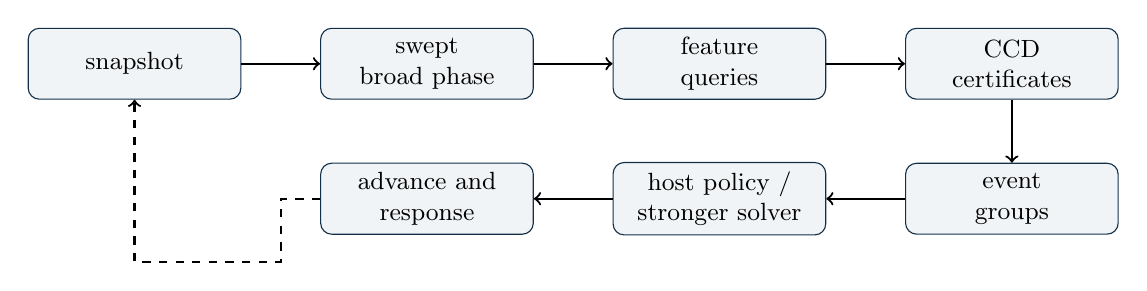
\begin{tikzpicture}[node distance=8mm and 10mm, every node/.style={font=\small}]
\tikzstyle{box}=[draw=navy,rounded corners,fill=softgray,minimum width=27mm,minimum height=9mm,align=center]
\node[box] (snap) {snapshot};
\node[box,right=of snap] (broad) {swept\\broad phase};
\node[box,right=of broad] (feat) {feature\\queries};
\node[box,right=of feat] (ccd) {CCD\\certificates};
\node[box,below=of ccd] (event) {event\\groups};
\node[box,left=of event] (policy) {host policy /\\stronger solver};
\node[box,left=of policy] (advance) {advance and\\response};
\draw[->,thick] (snap)--(broad);
\draw[->,thick] (broad)--(feat);
\draw[->,thick] (feat)--(ccd);
\draw[->,thick] (ccd)--(event);
\draw[->,thick] (event)--(policy);
\draw[->,thick] (policy)--(advance);
\draw[->,thick,dashed] (advance.west) -| ++(-.5,-.8) -| (snap.south);
\end{tikzpicture}
\caption{Host-owned integration sequence and closed replay loop.}
\end{figure}

\section{Uncertainty policy}

For interactive graphics, a host might substep or route an inconclusive query to a stronger solver. For safety-oriented robotics or public infrastructure, the policy may require a conservative stop. The choice is application-specific, but the engine must make it explicit. The library does not decide that uncertainty is harmless.

\section{Scale and tolerance}

A fixed absolute tolerance is unsuitable across arbitrary unit scales. Integration should define a scene normalization or a combined tolerance such as
\[
  \tau=\tau_{abs}+\tau_{rel}L,
\]
where $L$ is a declared local scale. Any contact thickness used for cloth or shell geometry must remain distinct from numerical tolerance.

\chapter{Cradle-to-grave lifecycle}
\section{Gate register}

\begin{longtable}{p{0.13\textwidth}p{0.25\textwidth}p{0.52\textwidth}}
\caption{Cumulative lifecycle gates for v0.5}\label{tab:gates}\\
\toprule
Gate & Objective & v0.5 evidence\\
\midrule
\endfirsthead
\toprule
Gate & Objective & v0.5 evidence\\
\midrule
\endhead
G0 & Provenance & immutable v0.4 baseline, source register, vendored corpus README/license/hashes\\
G1 & Problem & literal engine CCD, affine feature profile, exclusions and status algebra\\
G2 & Formalization & cubic equations, distance-rate fallback, rigid envelopes, event relation\\
G3 & CPU reference & Python VF/EE implementation and C++ bounds/events/impulse translation\\
G4 & Verification & unit, synthetic, external corpus, inequality, conservation, fuzz, deterministic digest\\
G5 & Benchmark & raw CSV records, JSON summary, figures, environment capture\\
G6 & Acceleration & coefficient-stage CUDA skeleton; gate deliberately not passed\\
G7 & Integration & host ordering, uncertainty policy, response boundary\\
G8 & Operations & telemetry, budgets, replay identifiers, degraded modes\\
G9 & Maintenance & semantic-version and compatibility-sensitive fields\\
G10 & Retirement & archive, defect register, migration and default-disable criteria\\
\bottomrule
\end{longtable}

\section{Operations telemetry}

At minimum, operations should count queries by type and status, root counts, fallback invocations, interval expansions, queue maxima, condition indicators, event sizes, timing, and response routing. Telemetry must not contain unnecessary personal data. Scene snapshots should be content-addressed or otherwise reproducibly identified.

\section{Incident response}

A missed contact or non-deterministic result is an incident. Preserve the exact input snapshot, binary/source version, compiler and numeric mode, capacities, tolerance policy, certificate records, and host response. Minimize the scene, add the minimal case to regression, determine whether the defect is algorithmic or policy-related, and issue a release note with affected profiles.

\chapter{Adapter separation after the CCD turn}

\begin{longtable}{p{0.19\textwidth}p{0.25\textwidth}p{0.45\textwidth}}
\caption{Non-CCD materials remain independent adapter programs}\\
\toprule
Adapter & Reusable artifact & Evidence required before a domain claim\\
\midrule
\endfirsthead
\toprule
Adapter & Reusable artifact & Evidence required before a domain claim\\
\midrule
\endhead
Measurement / sensors & timeline, residual, certificate & calibration, units, uncertainty, traceability, drift\\
SAR / wave sensing & swept support, event interval & governing wave model, sensor transfer function, field validation\\
GPU / edge AI & bounded queues, replay & kernel equivalence, quality, memory, energy and thermal tests\\
Optical / photonic & operator chain, feedback & measured transfer matrix, precision, drift, conversion and energy\\
Quantum / Cross--Kerr & parity/event notation & Hamiltonian/channel, state preparation, noise, measurement, scaling\\
Chemical networks & graph and controller & stoichiometry, kinetics, conservation, thermodynamic accounting\\
Biological / medical & observations and residuals & causal mechanism, toxicology, preclinical replication, controlled trials\\
Fabrication & geometry and certificate interchange & process window, metrology, yield, reliability and packaging\\
Cosmology & boundary vocabulary & two explicit theories, observable map, entropy/dynamics correspondence\\
\bottomrule
\end{longtable}

A shared computational interface can be useful without implying a shared physical law. No medical treatment, quantum advantage, optical processor, or cosmological duality is established by this release.

\chapter{Risk and assurance case}
\section{Top risks}

\begin{longtable}{p{0.25\textwidth}p{0.12\textwidth}p{0.52\textwidth}}
\caption{v0.5 risk register}\\
\toprule
Risk & Severity & Control / next evidence\\
\midrule
\endfirsthead
\toprule
Risk & Severity & Control / next evidence\\
\midrule
\endhead
Clustered or multiple cubic root missed & high & interval/exact root isolation; adversarial corpus expansion\\
Tolerance changes classification & high & scale policy, tolerance sweep, exact predicates\\
Persistent coplanarity consumes budget & high & specialized 2D-in-plane solver and interval arithmetic\\
Host treats unresolved as miss & critical & integration contract, telemetry, safe degradation tests\\
Event grouping hides distinct times & medium & declared merge tolerance and stronger ordering when needed\\
Impulse example used as production response & high & namespace/document boundary and explicit exclusions\\
GPU changes status or ordering & high & CPU/GPU per-query differential replay before conformance\\
Third-party corpus provenance lost & medium & vendored license, README, hashes, manifest\\
Personal identifiers propagated & medium & omit from generated metadata; minimize operational logs\\
Universal-substrate language overclaims evidence & high & separate adapter table and independent validation gates\\
\bottomrule
\end{longtable}

\section{Assurance argument}

\claim{The release makes uncertainty externally visible.} \evidence{Statuses, TOI intervals, methods, reasons, traces, records, and digests are explicit.} \boundary{Visibility does not make the underlying floating-point solver exact.}

\claim{The release is reproducible from local evidence.} \evidence{Fixed seeds, vendored data, environment capture, scripts, raw records, and SHA-256 manifest are supplied.} \boundary{CPU timing and floating-point details may differ across platforms.}

\claim{The CCD core is insulated from unsupported substrate claims.} \evidence{Adapter evidence burdens are independently stated.} \boundary{Future documents must continue to preserve this separation.}

\chapter{Roadmap to v0.6}
\section{Exactness first}

The next release should replace heuristic floating-point root acceptance with interval arithmetic or exact-predicate root isolation, including multiple roots and persistent coplanarity. The central metric is reduction of false and unresolved outcomes on complete public corpora, not an increase in symbolic scope.

\section{Mesh pipeline}

A half-edge or indexed-triangle adapter must generate non-adjacent VF/EE candidates, filter shared topology, preserve feature identities, handle self-collision exclusions, and group simultaneous events. Broad phase and feature expansion require their own capacity certificates.

\section{Rotating and deforming motion}

Affine endpoints cover deforming linear trajectories, but rigid screw motion is not affine at every point. A future profile must either use conservative rigid bounds with refinement or derive a validated rotational feature solver. Deformable self-collision requires topology-aware candidate management and thickness policy.

\section{Independent comparison}

At least two established CCD implementations should be run on the same complete corpora with identical labels and reporting. Independent reproduction should occur before claiming application advantage or GPU conformance.

\chapter{Maintenance and retirement}
\section{Compatibility}

Changes to status semantics, TOI interval meaning, tolerance defaults, root acceptance, corpus parser order, or digest serialization are compatibility-relevant. Semantic versioning should separate additive metadata from result-changing algorithms.

\section{Retirement triggers}

A release should be retired or disabled by default after discovery of an unbounded false-negative defect, loss of provenance, irreproducible package hashes, an incompatible schema without migration, or replacement by an independently reproduced stronger implementation. The archive must retain the final binaries/sources, known-defect register, migration guide, and corpus evidence.

\section{Closing assessment}

v0.5 is a meaningful engineering continuation: the CCD core now reaches moving mesh features, explicit degeneracy handling, event intervals, and public evidence ingestion. Its strongest quality is not universality but disciplined boundedness. The remaining work is exactness, complete mesh integration, cross-library comparison, and CPU/GPU equivalence.

\appendix
\chapter{Reproduction commands}

\begin{lstlisting}[language=bash]
cd 12_v0_5_upgrade
export PYTHONPATH="$PWD/src"
python -m unittest discover -s tests -v
python benchmarks/run_validation.py
python tools/fuzz_parser.py
python examples/feature_ccd_demo.py

# Native smoke test
c++ -std=c++17 -O2 -Icpp/include \
  cpp/src/nhdf_ccd_v05.cpp cpp/tests/smoke.cpp \
  -o nhdf_ccd_v05_smoke
./nhdf_ccd_v05_smoke
\end{lstlisting}

The top-level release also contains a SHA-256 manifest and a ZIP integrity record. The report build reads the validation JSON rather than duplicating values manually.

\chapter{Certificate JSON schema}
\lstinputlisting[language={},caption={Machine-readable v0.5 certificate schema}]{../spec/certificate_v0_5.schema.json}

\chapter{Event JSON schema}
\lstinputlisting[language={},caption={Machine-readable event schema}]{../spec/event_v0_5.schema.json}

\chapter{Corpus parser excerpt}
\lstinputlisting[language=Python,caption={Exact-rational eight-row corpus parser}]{../src/nhdf_ccd_v05/corpus.py}

\chapter{Feature solver excerpt}
\lstinputlisting[language=Python,firstline=1,lastline=205,caption={Cubic construction, witnesses, and bounded fallback excerpt}]{../src/nhdf_ccd_v05/ccd.py}

\chapter{Validation log}
\lstinputlisting[language={},caption={Generated v0.5 validation log}]{../validation/RELEASE_VALIDATION_LOG.md}

\chapter{File inventory by extension}
\begin{table}[H]
\centering
\caption{Upgrade-directory inventory at report generation}
\begin{tabular}{lr}
\toprule
Extension & Files\\
\midrule
\input{file_inventory_rows.tex}
\bottomrule
\end{tabular}
\end{table}

\chapter{Source and evidence register}
\begin{longtable}{p{0.14\textwidth}p{0.33\textwidth}p{0.43\textwidth}}
\toprule
ID & Artifact & Role\\
\midrule
S1 & Original one-bit/parity/log-polar prompt-chain PDF & provenance of the operator vocabulary\\
S2 & NHDF Formal Specification v0.1 PDF & local zero-set, bounded-resource, failure, and conformance corrections\\
S3 & Commute/design transcript PDF & log-polar and CCD intuition; overstrong one-lookup claim superseded\\
S4 & Spherical--Cartesian PDF & wider substrate claims retained as separate adapters\\
B4 & NHDF--CCD Cradle-to-Grave v0.4 PDF/ZIP & preserved primitive/core baseline\\
C1 & Sample-Queries README and MIT license & public corpus format and legal provenance\\
C2 & Two \path{erleben-sliding-spike} CSV files & external VF/EE evidence subset\\
V5 & \path{validation_summary.json} and raw CSV records & executed v0.5 evidence\\
\bottomrule
\end{longtable}

\chapter{Part II separator}
\thispagestyle{empty}
\vspace*{45mm}
\begin{center}
{\Huge\bfseries\color{navy} Part II}\par
\vspace{8mm}
{\LARGE Preserved NHDF--CCD v0.4 baseline}\par
\vspace{14mm}
\begin{minipage}{0.78\textwidth}
The pages following this separator are the prior v0.4 PDF, preserved without rewriting. Its primitive solvers, lifecycle package, and limitations remain the baseline on which the v0.5 feature-contact addendum was built. Where v0.5 and v0.4 differ, the newer status, scope, and evidence statements govern the v0.5 release.
\end{minipage}
\end{center}
\vfill

\end{document}
